%%%%%%%%%%%%%%%%%%%%%%%%%%%%%%%%%%%%%%%%%%%%%%%%%%%%%%%%%%%%%%%%%%%%%%%
%%%%%%%%%%%%%%%%%%%%%%%%%%%%%%%%%%%%%%%%%%%%%%%%%%%%%%%%%%%%%%%%%%%%%%%
\deelmetoef{Module 2}{Apps maken met MIT App Inventor 2}{Module 2. Apps maken met MIT App Inventor 2}{Oplossingen module 2}{Oplossingen module 2}
%%%%%%%%%%%%%%%%%%%%%%%%%%%%%%%%%%%%%%%%%%%%%%%%%%%%%%%%%%%%%%%%%%%%%%%
%%%%%%%%%%%%%%%%%%%%%%%%%%%%%%%%%%%%%%%%%%%%%%%%%%%%%%%%%%%%%%%%%%%%%%%

\begin{samenvatting}
We gaan een hartslagmonitor maken in de vorm van een smartphone app!
%De hartslagmonitor die we gaan maken is een smartphone app. 
MIT, een bekende universiteit in de Verenigde Staten, ontwikkelde een programmeeromgeving waarmee je zeer eenvoudig apps kan maken en testen. In dit hoofdstuk bespreken we de belangrijkste structuren voor het maken van een app. Ook in andere programmeertalen en -omgevingen zal je deze structuren kunnen gebruiken.
\end{samenvatting}
%

%%%%%%%%%%%%%%%%%%%%%%%%%%%%%%%%%%%%%%%%%%%%%%%%%%%%%%%%%%%%%%%%%%%%%%%
\section{MIT App Inventor 2}
\label{sec:Mod2_Sec1}
%%%%%%%%%%%%%%%%%%%%%%%%%%%%%%%%%%%%%%%%%%%%%%%%%%%%%%%%%%%%%%%%%%%%%%%
%
Met behulp van MIT App Inventor 2 kan je zelf apps maken. Alles wat je nodig hebt, is een computer met wifi-verbinding en een smartphone geconnecteerd met hetzelfde wifi-netwerk.

\subsection{Maken van de app}

Surf naar de website \url{http://appinventor.mit.edu/explore/} en klik rechtsboven op \hl{\texttt{Create apps!}} Je zal moeten inloggen met een google account. Als je nog geen google account hebt, kan je die aanmaken via \url{https://accounts.google.com/signup}. Na succesvol aanmelden kom je op de pagina met je projecten terecht. 

Cre\"eer een nieuw project, noem het bvb. \textquotedblleft HelloWorld\textquotedblright, en klik erop om het project te openen. 

Je komt op het startscherm terecht. Er zijn twee \textquoteleft views\textquoteright. 

\subsubsection{Ontwerper view}

De eerste view is de \hl{\emph{ontwerper view}}, weergegeven in Figuur \ref{fig:view_designer}.

\figuurmetlabel[\label{fig:view_designer}]{width=.8\linewidth}{module2/overviewAI2_tabs}{Ontwerper view in MIT App Inventor 2. Overschakelen tussen views doe je rechtsbovenaan (groene rechthoek). Tabs zijn aangeduid in rood.}

In deze view kan je de componenten toevoegen die je zal zien op het scherm tijdens het uitvoeren van je app.
Een component kan zijn: een \hl{\texttt{knop (Engels: button)}}, een \hl{\texttt{label}}, een \hl{\texttt{tekstvak (Engels: textbox)}} enz.

\begin{minipage}{.3\linewidth}
	\gewonefiguur{width=\linewidth}{module2/palette}
\end{minipage}
\hspace{2cm}
\begin{minipage}{.5\linewidth}
	In de \hl{\emph{Palet}} tab (links) vind je alle componenten die je kan toevoegen. Je voegt componenten toe door ze vast te nemen en ze naar het scherm van de afgebeelde smartphone te slepen. 
\end{minipage}


\textbf{Wat kan je allemaal doen met deze componenten? }

\begin{minipage}{.3\linewidth}
	\gewonefiguur{width=\linewidth}{module2/layout}
\end{minipage}
\hspace{2cm}
\begin{minipage}{.5\linewidth}
	Je kan je componenten grafisch schikken door ze in een \hl{\texttt{Indeling Horizontaal}}, \hl{\texttt{Indeling Vertikaal}} of \hl{\texttt{TabelIndeling}} te plaatsen.
\end{minipage}

\begin{minipage}{.5\linewidth}
	Om een overzicht te kunnen houden, moet je al snel je componenten benoemen. Dit doe je in de tab \hl{\emph{Componenten}}
	door de component te selecteren en op \hl{\texttt{Rename}} te drukken.
\end{minipage}
\hspace{2cm}
\begin{minipage}{.3\linewidth}
	\gewonefiguur{width=\linewidth}{module2/components}
\end{minipage}

\begin{minipage}{.5\linewidth}
	Je zal de eigenschappen van de componenten ook wijzigen voor de specifieke taak die ze zullen krijgen. Dit doe je in de \hl{\emph{Eigenschappen}} tab helemaal rechts.
	
	Welke tekst moet op de knop staan? Wat is de lettergrootte? Wil je de tekst in een andere kleur weergeven? ... 
\end{minipage}
\hspace{2cm}
\begin{minipage}{.3\linewidth}
	\gewonefiguur{width=\linewidth}{module2/properties}
\end{minipage}

%De componenten zijn ingedeeld in categori\"en.
%\begin{enumerate}
%	\item Ten eerste is er de \emph{User interface}: dit zijn componenten waarmee de gebruiker kan interageren.
%	Dit is bijvoorbeeld een \texttt{knop (Engels: button)}, een \texttt{label}, een \texttt{text} enz. 
%	\item Via de categorie \emph{Layout} kan je componenten kan je groeperen m.b.v. \texttt{HorizontalArrangement}, \texttt{VerticalArrangement} of \texttt{TableArrangement}. 
%	\item De andere categori\"en en componenten laten we je zelf ontdekken. Als je wilt weten wat een component doet, kan je het vraagteken naast de component in de tab \emph{Palette} aanklikken voor een korte uitleg.
%\end{enumerate}
%
%Toegevoegde componenten kan je een naam geven onder de tab \emph{Components} door de component aan te klikken en op \emph{Rename} te drukken. In de tab \emph{Properties} (rechts) kan je de eigenschappen van de component veranderen: Welke tekst moet op de knop staan? Wat is de lettergrootte? Wil je de tekst in een andere kleur weergeven? ... 


\subsubsection{Blokken view}

De andere view is de \hl{\emph{blokken view}}, weergegeven in Figuur \ref{fig:view_block}.

\figuurmetlabel[\label{fig:view_block}]{width=.8\linewidth}{module2/uitlegAI_blocks}{Blokken view in MIT App Inventor 2.}

De \hl{\emph{ontwerper view}} kan je vergelijken met het dashboard van een auto. De bestuurder ziet er alles waarmee hij de wagen kan besturen.
Door over te gaan naar de \hl{\emph{blokken view}}, duiken we als het ware in de motorkap van de wagen. Hier gaan we de eigenlijke werking van de app programmeren.

Wat moet er gebeuren als je op de knop drukt? Misschien wil je de tekst in een label aanpassen, of wil je een andere afbeelding tonen. Er kan veel; wat je implementeert, hangt af van je verbeelding en van hoe jij wil dat de app zal werken.

\begin{opdracht}{Experimenteren met MIT App Inventor 2}
Ga na wat je allemaal kan doen in de programmeeromgeving. Welke componenten bestaan er allemaal? Welke eigenschappen kan je aanpassen?

\begin{itemize}
	\item Probeer een eerste app te maken met een knop waarop de tekst \textquotedblleft Zeg hallo\textquotedblright \ staat en een label zonder tekst. 
	\item Als je op de knop drukt, moet de tekst \textquotedblleft Hello world!\textquotedblright \ in het label verschijnen. 
\end{itemize}

Dit \textquotedblleft Hello world!\textquotedblright-programma is een van de simpelste programmatjes die je kan schrijven. Wanneer programmeurs een nieuwe programmeertaal aanleren, schrijven ze steeds \textquotedblleft Hello world!\textquotedblright-programma om te leren werken met de nieuwe taal, die we met een geleerder woord syntax noemen.
\end{opdracht}

\subsection{Testen en uitvoeren van de app}
Om de app te testen moet je de MIT App Inventor 2 Companion App (te vinden in de Google Play Store) installeren op je smartphone. 
Zorg ervoor dat je computer en smartphone met hetzelfde wifi-netwerk verbonden zijn. 
Klik op \hl{\texttt{Verbinden}}, linksboven op het scherm zoals aangeduid op de figuur.

\gewonefiguur{width=.8\linewidth}{module2/overviewAI2_connect}

Kies de eerste optie \hl{AI companion}. Er verschijnt een QR-code die je kan scannen met je smartphone met de MIT App Inventor 2 Companion App. De app opent op je smartphone (even geduld, nergens op klikken!), zodat je de werking van de app kan testen.

Zolang je smartphone  via wifi gekoppeld is aan de Companion App, verandert de app op je smartphone tegelijkertijd met de aanpassingen die je doorvoert op het scherm van je computer. Soms werkt dit echter niet zo goed. Breek dan de connectie met de smartphone af via \hl{\texttt{Verbinden $>$ Reset verbinding}} en maak de verbinding opnieuw via \hl{\texttt{Verbinden $>$ AI companion}}.

Als je de app die je ontworpen hebt getest hebt via de App Inventor 2 Companion App en de app aan de vereisten voldoet, kan je de app downloaden. Zo heb je een zelfstandig werkende app op je smartphone, zonder dat je een wifi-verbinding met je computer of de MIT ontwikkelomgeving nodig hebt. Dan hoef je ook niet meer steeds de QR code te scannen als je de app wilt gebruiken. De app kan je installeren via \hl{\texttt{Bouwen $>$ App (toon QR-code voor .apk)}}. Door een QR-code te scannen met je smartphone kan je het installatie-bestand (.apk) downloaden op je smartphone. Wanneer je het .apk-bestand opent, installeert de app.

\begin{opdracht}{Good morning app}
	\begin{minipage}{.1\linewidth}
	
\includegraphics[width=1.5cm]{inputs/opdracht}
	\vspace{5cm}
	\end{minipage}
	\begin{minipage}{.5\linewidth}
	 Toon \textquotedblleft Good morning!\textquotedblright \ in drie verschillende talen op het scherm, nl. Italiaans, Spaans en Duits. 
	 Zorg ervoor dat:
	 \begin{itemize}
	 	\item een klik op de \hl{\texttt{knopItaliaans}} \textquotedblleft Buongiorno!\textquotedblright toont
	 	\item een klik op de \hl{\texttt{knopSpaans}} \textquotedblleft Buenos dias!\textquotedblright toont
	 	\item een klik op de \hl{\texttt{knopDuits}} \textquotedblleft Guten Morgen!\textquotedblright toont
	 \end{itemize}
	\end{minipage}
	\begin{minipage}{.3\linewidth}
		\gewonefiguur{width=5cm}{module2/goedemorgenApp}
	\end{minipage}

	Het is belangrijk eerst goed na te denken welke componenten nodig zijn en hoe je het gewenste gedrag in code zal programmeren alvorens op de computer vanalles te doen. Bij opdrachten waarin code moet geschreven worden gebruiken we daarom volgende aanpak: we schrijven uit wat we willen bereiken in de DENK-kolom en denken na hoe we dit bekomen. De aanpak schrijven we uit in de DOE-kolom. 
	
	\begin{tabular}{c|L{8cm}|L{8cm}}
	& \multicolumn{1}{>{\centering\arraybackslash}m{80mm}|}{\textbf{DENK}}  & \multicolumn{1}{>{\centering\arraybackslash}m{80mm}}{\textbf{DOE}}  \\
	\hline
	1 & & Cre\"eer een nieuw project, genaamd \textquotedblleft Goedemorgen \textquotedblright.  \\
	\hline
	2 & \emph{Ontwerper} view: & \\
	&   Welke layout kies je? & De knoppen staan onder elkaar $\rightarrow$ \hl{\texttt{Indeling Verticaal}} \vspace{1cm}\\
	&   Welke componenten heb je nodig? & \vspace{2cm} \\
	&   Welke naam geef je aan iedere component? & \vspace{2cm} \\
	&  	Welke eigenschappen heeft elke component nodig? & \vspace{2cm} \\
	\hline
	3 & \emph{Blokken} view: \newline 
	Hoe zorg je ervoor dat: & \\
	& 1. een klik op de \hl{\texttt{knopItaliaans}} \textquotedblleft Buongiorno!\textquotedblright toont  & \\
	& & 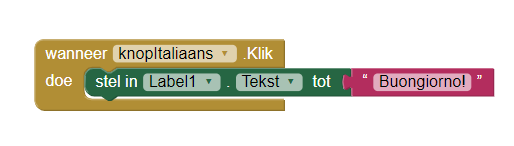
\includegraphics[width=\linewidth]{inputs/module2/goedemorgen_italiaans} \\
	&  2. een klik op de \hl{\texttt{knopSpaans}} \textquotedblleft Buenos dias!\textquotedblright toont & 
	\vspace{2cm} \\
	&  3. een klik op de \hl{\texttt{knopDuits}} \textquotedblleft Guten Morgen!\textquotedblright toont & 
	\vspace{2cm} \\
	\end{tabular}

Test de werking van je app grondig. Doet de app op elk moment wat je ervan verwacht? Indien niet, ga dan op zoek naar de onderliggende oorzaak. Het proces waarin je ongewenste fouten in de werking van de app opspoort en wegwerkt, heet \textquotedblleft debuggen \textquotedblright. Zelfs de beste programmeurs moeten hun apps debuggen. Dit is soms een frustrerend proces, maar het is helaas wel een wezenlijk onderdeel van programmeren.

\opdrachteindbalk

\end{opdracht}

%%%%%%%%%%%%%%%%%%%%%%%%%%%%%%%%%%%%%%%%%%%%%%%%%%%%%%%%%%%%%%%%%%%%%%%
\section{Blokken in de blokken view}
\label{sec:Mod2_Sec2}
%%%%%%%%%%%%%%%%%%%%%%%%%%%%%%%%%%%%%%%%%%%%%%%%%%%%%%%%%%%%%%%%%%%%%%%
%
Met MIT App Inventor 2 kan je heel gemakkelijk zelf aan de slag. De betekenis van de componenten is vaak intu\"itief duidelijk en via het vraagteken kan je steeds extra uitleg oproepen. 

Hieronder bespreken we enkele belangrijke blokken uit de blocks view, waarvan de bedoeling misschien iets minder vanzelfsprekend is.

\subsection{Variabelen (Variables)}
Variabelen worden gebruikt om waarden bij te houden. Een bij te houden waarde kan bvb. het resultaat van een wiskunde bewerking zijn, of een tekst input van de gebruiker die je later nog wilt aanpassen. 

Belangrijk is dat er een onderscheid gemaakt wordt tussen \emph{lokale} en \emph{globale} variabelen, zie Figuur \ref{fig:variabele}. Globale variabelen worden aangemaakt bij de opstart van het programma en kunnen doorheen het hele programma gebruikt worden. We zouden kunnen zeggen dat je vanuit elk blok \textquotedblleft aan de globale variabele kan\textquotedblright.
Lokale variabelen worden aangemaakt binnen een blok en kunnen enkel door blokken binnen de grenzen van de lokale variabele gebruikt worden. Je \textquotedblleft kan er dus enkel aan\textquotedblright \ binnen het oranje blok zelf. Vandaar dat het blok voor een lokale variabele onderaan nog een oranje staartje heeft. Dit staartje duidt aan binnen welke grenzen \textquotedblleft je aan de variabele kan\textquotedblright.

\figuurmetlabel[\label{fig:variabele}]{width=8cm}{module2/variabelen}{Het bovenste blok toont hoe je een globale variabele kan aanmaken, die doorheen het hele programma gebruikt kan worden. Het onderste blok toont hoe je een lokale variabele kan aanmaken, die enkel toegankelijk is binnen het blok van de variabele.}

De \hl{\texttt{Krijg}}-instructie wordt gebruikt om de waarde van een variabele op te halen. De \hl{\texttt{Zet}}-instructie wordt gebruikt om de waarde van een variabele te wijzigen.

\subsection{Controle (control)}
De meeste programmeertalen zijn opgebouwd rond drie belangrijke controlestructuren: 

\begin{enumerate}
	\item \textquoteleft Als dan\textquoteright-testen om beslissingen te nemen, 
	\item \textquoteleft Voor elke\textquoteright-lussen om herhaling in te bouwen, en
	\item  \textquoteleft Terwijl \textquoteright-lussen om herhaling in te bouwen.
\end{enumerate}

\subsubsection{Beslissingen nemen: \emph{Als dan} blok}

\begin{minipage}{.5\linewidth}
\gewonefiguur{width=7cm}{module2/if.jpg}
\end{minipage}
\begin{minipage}{.5\linewidth}
\gewonefiguur{width=7cm}{module2/ifStructures}
\end{minipage}

\hl{\texttt{Als dan}}-testen laten toe een programma dynamisch te maken. Een \hl{\texttt{Als dan}}-test kan je vergelijken met het kiezen van een weg op een kruispunt: als een voorwaarde voldaan is (YES), ga je naar links; anders (NO) ga je rechts. 

Het testen of een voorwaarde voldaan is, gebeurt met een \texttt{Boolean} expressie.
Een \texttt{Boolean} expressie is een uitdrukking die ofwel waar of ofwel vals is.
Het resultaat van \texttt{Boolean} expressie is een \texttt{Boolean}, een variabele die maar twee waarden kan aannemen: \texttt{true} als de voorwaarde voldaan is, en \texttt{false} als de voorwaarde niet voldaan is.

In App Inventor zijn er verschillende implementaties van deze structuur mogelijk:
\begin{itemize}
	\item \emph{Als dan} blok \\
	\begin{minipage}{.5\linewidth}
	Je kan kiezen om een bewerking enkel uit te voeren als een voorwaarde voldaan is (\hl{\texttt{Als dan}} blok).
	\end{minipage}
	\begin{minipage}{.5\linewidth}
	\gewonefiguur{height=2cm}{module2/ifthen}
	\end{minipage}	
	\item \emph{Als dan anders} blok \\
	\begin{minipage}{.5\linewidth}
			Het kan zijn dat je een eerste bewerking wenst uit te voeren als aan de voorwaarde voldoaan is, maar dat er een andere bewerking zal gebeuren indien nodig. De \textquotedblleft else\textquotedblright \ toevoegen doe je door op het blauwe icoontje met het tandwieltje te klikken en een \textquotedblleft else\textquotedblright -blokje in het \hl{\texttt{Als dan}}-blok te slepen.
	\end{minipage}
	\begin{minipage}{.5\linewidth}
		\gewonefiguur{height=6cm}{module2/ifelse}
	\end{minipage}	
	\item \emph{Als dan, of als dan, anders dan} blok \\
	\begin{minipage}{.5\linewidth}
		Als je echt complexe dingen wil doen, kan je extra voorwaarden toevoegen. Dit doe je door op het blauwe icoontje met het tandwieltje te klikken en \textquotedblleft else if\textquotedblright -blokjes en een \textquotedblleft else\textquotedblright -blokje in het \hl{\texttt{Als dan}}-blok te slepen..
	\end{minipage}
	\begin{minipage}{.5\linewidth}
		\gewonefiguur{height=8cm}{module2/ifelseifelse}
	\end{minipage}	
\end{itemize}

\begin{opdracht}{Gemiddelde app}
	\begin{minipage}{.1\linewidth}
		
\includegraphics[width=1.5cm]{inputs/opdracht}
		\vspace{3cm}
	\end{minipage}
	\begin{minipage}{.5\linewidth}
		De gebruiker geeft drie getallen in. Bij het indrukken van de knop wordt het gemiddelde van de drie getallen berekend en in het onderste tekstvak geplaatst. Als het gemiddelde hoger is dan 95, wordt de tekst \textquotedblleft Mooi gedaan  \textquotedblright \ weergegeven in het bovenste label. Bij het indrukken van de knop worden alle velden opnieuw op hun oorspronkelijke waarde gezet.
	\end{minipage}
	\begin{minipage}{.3\linewidth}
		\gewonefiguur{width=5cm}{module2/gemiddeldeApp}
	\end{minipage}
	
	\begin{tabular}{c|L{8cm}|L{8cm}}
		& \multicolumn{1}{>{\centering\arraybackslash}m{80mm}|}{\textbf{DENK}}  & \multicolumn{1}{>{\centering\arraybackslash}m{80mm}}{\textbf{DOE}}  \\
		\hline
		1 & & Cre\"eer een nieuw project, genaamd \textquotedblleft Gemiddelde\textquotedblright.  \\
		\hline
		2 & \emph{Ontwerper} view: & \\
		&   1. Welke layout kies je? & \\
		&   2. Welke componenten heb je nodig? & \vspace{2cm} \\
		&   3. Welke naam geef je aan iedere component? & \vspace{2cm} \\
		&  	4. Welke eigenschappen heeft elke component nodig? & \vspace{2cm} \\
		\hline
		3 & \emph{Blokken} view: \newline 
		Hoe zorg je ervoor dat: & \\
		&  1. een lokale variabele gemiddelde aangemaakt wordt? & \\
		& & 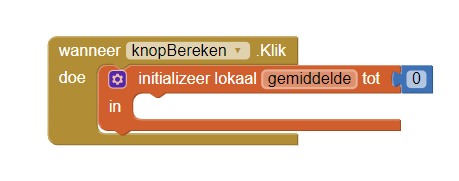
\includegraphics[width=\linewidth]{inputs/module2/gemiddeldeLokaal} \\
		&  2. het gemiddelde berekend wordt? & 
		\vspace{2cm} \\
		&  3. het gemiddelde in het juiste tekstvak getoond wordt? & 
		\vspace{2cm} \\
		& 4. \textquotedblleft Mooi gedaan! \textquotedblright getoond wordt als het gemiddelde groter is dan 95? & \vspace{2cm} \\
	\end{tabular}
	
	Test de werking van je app grondig. 
	
	\opdrachteindbalk
	
\end{opdracht}

\subsubsection{Herhaling: \emph{Terwijl test} lus of \emph{for each} lus}

Voor zaken die je veelvuldig wil uitvoeren, kan je gebruik maken van een een repetitie-blok, zoals een \hl{\texttt{Terwijl test}}-lus of \hl{\texttt{Voor elke}}-lus. 
Zo'n herhaling zou kunnen zijn: de tekst op een label laten optellen van 1 tot 100.

\gewonefiguur{width=\linewidth}{module2/repititionStructures2}

\begin{itemize}
	\item Bij een \hl{\texttt{Voor elke}}-lus wordt een \emph{teller} (in ons voorbeeld \texttt{getal}) steeds verhoogd (in ons voorbeeld met $Z$) binnen een bereik van waarden (in ons voorbeeld tussen $X$ en $Y$). Een \\hl{\texttt{Voor elke}}-lus is ideaal om een probleem op te lossen waarbij een lus een vast aantal keer herhaald moet worden.

	\item Een \hl{\texttt{Terwijl test}}-lus heeft twee delen: 
	\begin{enumerate}
		\item een \hl{\texttt{Terwijl test}}-socket: \texttt{Boolean} expressie (waar of niet waar?) die getest wordt, en 
		\item een \hl{\texttt{doe}}-socket: een verzameling instructies die uitgevoerd wordt zolang de \texttt{Boolean} expressie \texttt{true} is.
	\end{enumerate}
	Bij het programmeren van een herhalingslus moet de booleaanse uitdrukking ooit \texttt{false} worden. Anders blijft het programma eindeloos in cirkeltjes draaien en zal het lijken alsof er niets gebeurt, ook al is de computer aan het rekenen!
	Pas dus op dat je geen oneindige lussen maakt: ooit moet de \texttt{Boolean} expressie \texttt{false} worden, anders blijf je vastzitten in de \hl{\texttt{Terwijl test}}-lus!!!
\end{itemize}

\begin{opdracht}{Sommeer getallen app}
	\begin{minipage}{.1\linewidth}
		
\includegraphics[width=1.5cm]{inputs/opdracht}
		\vspace{1cm}
	\end{minipage}
	\begin{minipage}{.5\linewidth}
		Bereken de som van de getallen tussen nul en een bovengrens die de gebruiker ingeeft.
	\end{minipage}
	\begin{minipage}{.3\linewidth}
		\gewonefiguur{width=5cm}{module2/sommeerGetallen}
	\end{minipage}
	
	\begin{tabular}{c|L{8cm}|L{8cm}}
		& \multicolumn{1}{>{\centering\arraybackslash}m{80mm}|}{\textbf{DENK}}  & \multicolumn{1}{>{\centering\arraybackslash}m{80mm}}{\textbf{DOE}}  \\
		\hline
		1 & & Cre\"eer een nieuw project, genaamd \textquotedblleft Sommeer getallen\textquotedblright.  \\
		\hline
		2 & \emph{Ontwerper} view: & \\
		&  1. Welke layout kies je? & \\
		&  2. Welke componenten heb je nodig? & \vspace{2cm} \\
		&  3. Welke naam geef je aan iedere component? & \vspace{2cm} \\
		&  4. Welke eigenschappen heeft elke component nodig? & \vspace{2cm} \\
		\hline
		3 & \emph{Blokken} view: & \\
		&  1.  Maak een lokale variabele \texttt{Totaal} aan.& 1. Maak een lokale variabele \texttt{Totaal} aan. \vspace{.5cm}\\
		& 2. Beslis of je met een \hl{\texttt{Voor elke}}-lus of met een \hl{\texttt{Terwijl test}}-lus wilt werken. Beide kunnen, maar een \hl{\texttt{Voor elke}}-lus is hier net iets eenvoudiger. \vspace{.5cm} & \\
		&  3. Stel de \hl{\texttt{Voor elke}}-lus correct in. & 
		\vspace{2cm} \\
		&  4. Welke code moet binnen de lus uitgevoerd worden? Herinner je dat we telkens getallen bij de variabele \texttt{Totaal} willen optellen.  & 
		\vspace{2cm} \\
		&  5. Geef de waarde van de variabele \texttt{Totaal} weer in het tekstvak. & 4. Geef de waarde van de variabele \texttt{Totaal} weer in het tekstvak.\\
	\end{tabular}
	
	Test de werking van je app grondig. 
	
	\opdrachteindbalk
	
\end{opdracht}

\begin{opdracht}{Sommeer getallen app}
	\begin{minipage}{.1\linewidth}
		
\includegraphics[width=1.5cm]{inputs/opdracht}
		\vspace{1cm}
	\end{minipage}
	\begin{minipage}{.5\linewidth}
		Ontwikkel een app die het \texttt{Eindbedrag} berekent van een \texttt{Startbedrag} dat gedurende een \texttt{aantalJaar} op de bank staat tegen een bepaalde \texttt{rentevoet}.
	\end{minipage}
	\begin{minipage}{.3\linewidth}
		\gewonefiguur{width=5cm}{module2/intrestApp}
	\end{minipage}

	Je krijgt interest op een bedrag dat gedurende een jaar op de bank heeft gestaan. Hoeveel interest je krijgt, hangt af van de rentevoet. De rentevoet wordt meestal in percent uitgedrukt. Vroeger waren er hoge rentevoeten van rond de 5\%, maar tegenwoordig zijn de rentevoeten gedaald naar hele lage waarden rond de 0.1\%. 
	
	Als een bedrag $b$ een jaar op je rekening stond tegen een rentevoet $r$, levert dat je een eindbedrag $B$ op:
	\begin{equation*}
	B = b(1+r)
	\end{equation*}
	In deze formule moet je $r$ als kommagetal schrijven, dus $r=0.05$ voor een rentevoet van 5\%.
	
	\begin{tabular}{c|L{8cm}|L{8cm}}
		& \multicolumn{1}{>{\centering\arraybackslash}m{80mm}|}{\textbf{DENK}}  & \multicolumn{1}{>{\centering\arraybackslash}m{80mm}}{\textbf{DOE}}  \\
		\hline
		1 & & Cre\"eer een nieuw project, genaamd \textquotedblleft Sommeer getallen\textquotedblright.  \\
		\hline
		2 & \emph{Ontwerper} view: & \\
		&  1. Welke layout kies je? & \\
		&  2. Welke componenten heb je nodig? & \vspace{2cm} \\
		&  3. Welke naam geef je aan iedere component? & \vspace{2cm} \\
		&  4. Welke eigenschappen heeft elke component nodig? & \vspace{2cm} \\
		\hline
		3 & \emph{Blokken} view: & \\
		&  1.  Maak een lokale variabele \texttt{Eindbedrag} aan. Wat is een goede startwaarde? \vspace{.5cm} &  \\
		& 2. Maak een lokale variabele \texttt{Factor} aan. Dat is de waarde waarmee het bedrag op je rekening op het einde van elk jaar vermenigvuldigd wordt. \newline \emph{Hint:} de factor is gerelateerd aan de rentevoet $r$. \vspace{.5cm} & \\
		&  3. Verhoog het eindbedrag op het einde van elk jaar. Welk soort lus zal je hiervoor gebruiken? \newline
		\emph{Hint:} beide types lussen kunnen gebruikt worden; probeer ze allebei eens uit! & 
		\vspace{3cm} \\
		&  4. Geef de waarde van de variabele \texttt{Eindbedrag} weer in het tekstvak. & 4. Geef de waarde van de variabele \texttt{Eindbedrag} weer in het tekstvak.\\
	\end{tabular}
	
	Test de werking van je app grondig. 
	
	\opdrachteindbalk
\end{opdracht}

\subsection{Logica (Logic)}

Zoals eerder gezegd is een \texttt{Boolean} expressie een expressie die ofwel waar of ofwel vals is.
We kunnen op een aparte manier gaan rekenen met de mogelijkheden waar en vals.
Hiervoor beschikken we over zogenaamde \textquoteleft logische operatoren\textquoteright. 
Dit zijn bewerkingen waarmee we booleaanse uitdrukkingen kunnen combineren.
Zo kunnen we meer complexe voorwaarden testen. 

\begin{itemize}
	\item De logische operator \texttt{AND} geeft als output waar als \textbf{beide} inputs waar zijn, en onwaar als een of meerdere inputs onwaar zijn. 

	\item De logische operator \texttt{OR} geeft als output waar als \textbf{minstens \'e\'en} van beide inputs waar is, en onwaar als \textbf{beide} inputs onwaar zijn.
	
	\item De logische operator \texttt{NOT} geeft als output onwaar als de \textbf{input waar is} en geeft als output waar als de \textbf{input onwaar is}.
\end{itemize}

\subsection{Wiskunde (Math)}
Uiteraard kunnen bewerkingen op getallen uitgevoerd worden. Je vindt het volledige overzicht van mogelijke bewerkingen onder \emph{Bloken - wiskunde}.

\subsection{Tekst (Text)}
Naast wiskundige bewerkingen kan je ook tekst input van de gebruiker verwerken. De mogelijke bewerkingen die je op tekst kan uitvoeren vind je onder \emph{Blokken - Tekst}.


\subsection{Lijsten (Lists)}
Een lijst kan meerdere items met gelijkaardige data bevatten. Zo kan je bijvoorbeeld een lijst van getallen hebben, of een lijst van tekstwaarden. Als je 100 getallen moet bijhouden, is het makkelijker een lijst te gebruiken dan 100 verschillende variabelen.

Nadat een lijst wordt aangemaakt zoals in Figuur \ref{fig:lijst}, kan je extra items aan de lijst toevoegen, of er items uit verwijderen. De volledige lijst van bewerkingen die je op een lijst kan toepassen, vind je onder \emph{Blokken - Lijst}.

\figuurmetlabel[\label{fig:lijst}]{width=8cm}{module2/lijst}{Je kan een lege lijst aanmaken (boven), of een lijst aanmaken die reeds een aantal elementen bevat (onder).}

\begin{opdracht}{Boodschappenlijstje app}
	\begin{minipage}{.1\linewidth}
		
\includegraphics[width=1.5cm]{inputs/opdracht}
		\vspace{1cm}
	\end{minipage}
	\begin{minipage}{.5\linewidth}
		Maak een lijst met boodschappen aan. Print de lijst af op het scherm. Voeg een item toe aan de lijst, vervang een item uit de lijst en verwijder een item uit de lijst.
	\end{minipage}
	\begin{minipage}{.3\linewidth}
		\gewonefiguur{width=\linewidth}{module2/boodschappenlijst}
	\end{minipage}
	
	\begin{tabular}{c|L{8cm}|L{8cm}}
		& \multicolumn{1}{>{\centering\arraybackslash}m{80mm}|}{\textbf{DENK}}  & \multicolumn{1}{>{\centering\arraybackslash}m{80mm}}{\textbf{DOE}}  \\
		\hline
		1 & & Cre\"eer een nieuw project, genaamd \textquotedblleft Boodschappenlijst\textquotedblright.  \\
		\hline
		2 & \emph{Ontwerper} view: & \\
		&  1. Welke layout kies je? & \\
		&  2. Welke componenten heb je nodig? & \vspace{2cm} \\
		&  3. Welke naam geef je aan iedere component? & \vspace{2cm} \\
		&  4. Welke eigenschappen heeft elke component nodig? & \vspace{2cm} \\
		\hline
		3 & \emph{Blokken} view: & \\
		&  1.  Maak een globale variabele \texttt{boodschappenLijst} aan, die boodschappen bevat. \vspace{.2cm} &  \\
		& 2. Toon de lijst op het scherm. \vspace{.5cm} & \\
		& 3. Voeg een item toe aan de lijst. & 
		\vspace{1cm} \\
		& 4. Verwijder een item uit de lijst. & 
		\vspace{1cm} \\
		& 5. Vervang een item uit de lijst door een ander item. & 
		\vspace{1cm} \\
	\end{tabular}
	
	Test de werking van je app grondig. 
	
	\opdrachteindbalk
	
\end{opdracht}

